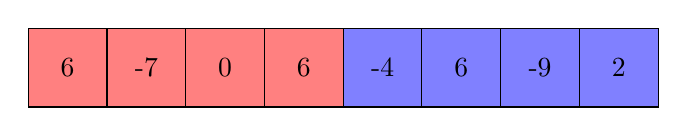
\begin{tikzpicture}
    % Define hardcoded values
    \def\values{6, -7, 0, 6, -4, 6, -9, 2}
    \foreach [count=\i from 0] \val in \values {
      \ifnum\i<4
        \definecolor{blockcolor}{rgb}{1,0.5,0.5} % light red
      \else
        \definecolor{blockcolor}{rgb}{0.5,0.5,1} % light blue
      \fi
  
      % Draw colored block
      \fill[blockcolor] (\i,0) rectangle ++(1,1);
      \draw (\i,0) rectangle ++(1,1);
      \node at (\i+0.5,0.5) {\val};
    }
  \end{tikzpicture}
  